\chapter{Übergreifende Aspekte der Realisierung}
\label{cha:realisierung}
In diesem Kapitel werden allgemeine Komponenten für die Umsetzung dieses Projektes beschrieben. Dabei werden jeweils nur die Techniken vorgestellt, welche von mehreren Komponenten genutzt werden, sodass sie in den jeweils dafür vorgesehenen Kapiteln nicht mehrfach genannt werden müssten. Abbildung \ref{pic:architecture-detailed} zeigt hier bei die genutzten Produkte zu den definierten Komponenten aus Kapitel \ref{sec:programmarchitektur}. Begriffe, welche nur in einem Teilbereich des Systems (Server oder einer der Clients) genutzt werden, werden in den jeweiligen Kapiteln gesondert besprochen).
\begin{figure}[!h]
\centering
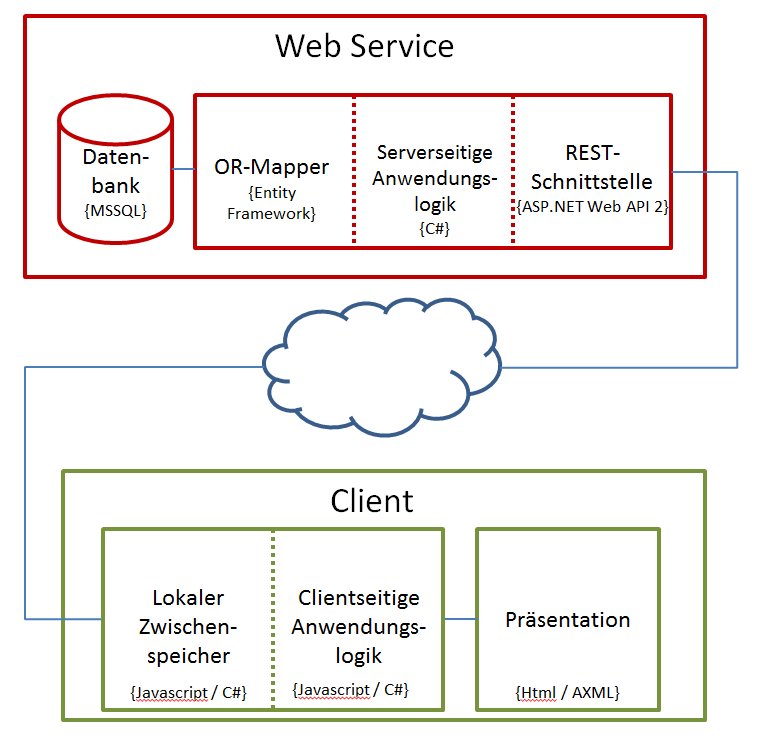
\includegraphics[width=0.7\linewidth]{content/images/Aufbau-Architektur-detailliert.png}
\caption{Zuordnung von Produkten und Techniken zu Verantwortlichkeiten}
\label{pic:architecture-detailed}
\end{figure}
Als Leitfaden wird versucht, möglichst viele Entwicklungswerkzeuge eines Unternehmens zu benutzen, um positive Synergieeffekte, beispielsweise in Form von leichter Kommunikation, zwischen den gewählten Komponenten zu gewährleisten. Zur Umsetzung dieses Projekts werden weitestgehend Produkte der Softwarefirma \textit{Microsoft} genutzt.
\newpage
\section{Datenbank-System}
\label{sec:DB-System}
Als Datenbanksystem wird die Lösung von \textit{Microsoft} verwendet. Hierbei handelt es sich um \textit{\ac{MSSQL}}. Durch die einheitliche Nutzung von \textit{Microsoft}-Produkten kann für den Zugriff auf die Datenbank der \ac{OR-Mapper} genutzt werden. Dieser erlaubt es, direkt aus Modell-Klassen Datenbank-Entitäten zu entwickeln. Dieser Vorgang wird in Kapitel \ref{ssec:aufbau-server-db} näher erläutert.\footcite{online:SQLServer}
\section{Hosting-Plattform}
\label{sec:Hosting-Plattform}
Sowohl der Web Service als auch der \ac{SPA}-Client müssen im Internet verfügbar gemacht werden, damit sie so von überall erreichbar sind. Hierzu bietet \textit{Microsoft} die Hosting-Plattform \textit{Azure} an. Diese ermöglicht es, direkt aus \textit{\ac{Visual Studio}} heraus, seine Webanwendung zu veröffentlichen. Gleichzeitig lässt sich eine Datenbank hosten, welchen der Web Service direkt benutzen kann. Zusätzlich ist \textit{Azure} sehr gut skalierbar, was den Einsatz als Hosting-Plattform für kleine Prototyp-Projekte optimal unterstützt.\footcite{online:Azure}
\section{Entwicklungsumgebung}
\label{sec:entwicklungsumgebung}
Für die Entwicklung sämtlicher Komponenten wird \textit{\ac{Visual Studio}} benutzt. Hierbei handelt es sich um die Standard-Entwicklungsplattform von \textit{Microsoft}. Diese Entscheidung wurde aus folgenden Gründen getroffen:
\begin{itemize}
\item Die Clients sollen durch zwei Drittanbieter-Frameworks umgesetzt werden, um den Implementierungsaufwand zu verringern. Eine genauere Erläuterung der Funktionsweise, der Vorteile und der Einbindung werden in den Kapiteln \ref{cha:native-app} und \ref{cha:web-app} gegeben. Beide Frameworks sind entweder bereits in die Entwicklungsumgebung integriert oder können problemlos nachträglich zum Projekt hinzugefügt werden. Die hierfür benutzten Programmiersprachen \textit{\gls{C-sharp}} und \textit{\gls{Javascript}} werden vollständig mit gängigen Features einer \ac{IDE}, wie Autovervollständigung, Syntax-Highlighting und Debugger, unterstützt. 
\item Die Entwicklung von Web Anwendungen wird stark erleichtert, da \ac{Visual Studio} mit einem integrierten Web Server ausgeliefert wird. Dadurch können entwickelte Applikationen direkt lokal getestet werden, ohne, dass ein zusätzlicher Web Server installiert oder die Anwendung auf einen Web Server veröffentlicht werden muss.
\item Es besteht eine starke Integration zu anderen \textit{Microsoft} Produkten. Hierzu zählen die Hosting-Plattform \textit{Microsoft Azure} und das Datenbank-System \textit{\ac{MSSQL}}.
\item Die Entwicklungsumgebung kann benötigte Komponenten und deren Abhängigkeiten durch den integrierten Paketmanager \gls{NuGet} nachladen. Dadurch entfällt das nachträgliche Herunterladen von \textit{\ac{DLL}}-Dateien, wodurch Kompatibilitätsprobleme verringert werden.\footcite{online:VisualStudio}
\end{itemize}
\section{Dokumentationslösung}
\label{sec:dokumentationslösung}
Zur Umsetzung der Projektdokumentation wird das Framework \textit{LaTeX} benutzt. Dieses erweitert das Textsatzsystem \textit{Tex} mit \glspl{Makro}. Die \glspl{Makro} können als \gls{Markup} benutzt werden, um einen Text zu strukturieren. Dadurch kann, wie bei Nutzung von \gls{Markup} üblich, sehr einfach Inhalt und Aussehen getrennt werden. Somit hat man den Vorteil, dass man nur einmal das Aussehen pflegen muss und anschließend ausschließlich den Inhalt mit dem gewünschten \gls{Markup} definieren muss. Diese Dateien können nachfolgend zu einer \textit{PDF}-Datei kompiliert werden.\footcite{online:definition-latex}\\ 
Ein weiterer Vorteil ist, dass die Inhaltsdateien aus einfachen Textdateien bestehen. Bei dieser Art von Dateien lassen sich Änderungen (z.B. Mittels Versionsverwaltung) leichter nachvollziehen als beispielsweise bei \textit{DOCX}-Dateien, welche das Textverarbeitungsprogramm \textit{Microsoft Word} benutzt. Dabei handelt es sich um Binärdateien, welche die Nachvollziehbarkeit erschweren.
\section{Versionsverwaltung}
\label{sec:versionsverwaltung}
Dieses Projekt wird von mehren Personen durchgeführt. Dabei ist es unerlässlich, dass die Projektstände zwischen den Teilnehmern nachvollziehbar verwaltet werden, da sonst schnell die Übersicht verloren gehen kann. Um dem entgegenzuwirken wird \textit{Git} zur Versionsverwaltung eingesetzt. \\
Diese Entscheidung wurde aus folgenden Gründen getroffen:
\begin{itemize}
\item \textit{Git} ist ein verteiltes Versionsverwaltungssystem. Das bedeutet, dass sowohl ein lokales- als auch ein globales Repository entsteht. Dies macht die Entwicklung leichter: Im vorliegenden Fall wird beispielsweise solange lokal entwickelt, bis eine Funktionalität vollständig implementiert und getestet ist. Anschließend werden alle lokalen Stände in das globale Repository eingecheckt, sodass immer ein funktionierender Stand im globalen Repository vorliegt. \footcite{online:definition-git}
\item Für die Nutzung von \textit{Git} benötigt man keinen eigenen Server, in dem das globale Repository aufgespielt wird. Hierfür kann die Webseite \href{https://github.com}{\textit{https://github.com}} genutzt werden. Diese stellt diese Funktionalität kostenlos bereit und ist weltweit über das Internet verfügbar. 
\item Für \textit{Git} gibt es eine direkte Integration in die \ac{Visual Studio}.
\end{itemize}